%%%%%%%%%%%%%%%%%%%%%%%%%%%%%%%%%%%%%%%%%%%%%%%%%%%%%%%%%%%%%%%%%%%%%%%%%%%%%%%%%%%%%%%%%%%%%%%%%%%%%%%%%%%%%%%%%%%%%%%%%%%%%%%%%%%%%%%%%%%%%%%%%%%%%%%%%%%
% This is just an example/guide for you to refer to when submitting manuscripts to Frontiers, it is not mandatory to use Frontiers .cls files nor frontiers.tex  %
% This will only generate the Manuscript, the final article will be typeset by Frontiers after acceptance.   
%                                              %
%                                                                                                                                                         %
% When submitting your files, remember to upload this *tex file, the pdf generated with it, the *bib file (if bibliography is not within the *tex) and all the figures.
%%%%%%%%%%%%%%%%%%%%%%%%%%%%%%%%%%%%%%%%%%%%%%%%%%%%%%%%%%%%%%%%%%%%%%%%%%%%%%%%%%%%%%%%%%%%%%%%%%%%%%%%%%%%%%%%%%%%%%%%%%%%%%%%%%%%%%%%%%%%%%%%%%%%%%%%%%%

%%% Version 3.4 Generated 2022/06/14 %%%
%%% You will need to have the following packages installed: datetime, fmtcount, etoolbox, fcprefix, which are normally inlcuded in WinEdt. %%%
%%% In http://www.ctan.org/ you can find the packages and how to install them, if necessary. %%%
%%%  NB logo1.jpg is required in the path in order to correctly compile front page header %%%

\documentclass[utf8]{FrontiersinHarvard}

%\setcitestyle{square} % for Physics and Applied Mathematics and Statistics articles
\usepackage{url,hyperref,lineno,microtype,subcaption}
\usepackage[onehalfspacing]{setspace}

\linenumbers


% BELOW TAKEN FROM rticles plos template
%
% amsmath package, useful for mathematical formulas
\usepackage{amsmath}
% amssymb package, useful for mathematical symbols
\usepackage{amssymb}

% hyperref package, useful for hyperlinks
\usepackage{hyperref}

% graphicx package, useful for including eps and pdf graphics
% include graphics with the command \includegraphics
\usepackage{graphicx}

% Sweave(-like)
\usepackage{fancyvrb}
\DefineVerbatimEnvironment{Sinput}{Verbatim}{fontshape=sl}
\DefineVerbatimEnvironment{Soutput}{Verbatim}{}
\DefineVerbatimEnvironment{Scode}{Verbatim}{fontshape=sl}
\newenvironment{Schunk}{}{}
\DefineVerbatimEnvironment{Code}{Verbatim}{}
\DefineVerbatimEnvironment{CodeInput}{Verbatim}{fontshape=sl}
\DefineVerbatimEnvironment{CodeOutput}{Verbatim}{}
\newenvironment{CodeChunk}{}{}

% cite package, to clean up citations in the main text. Do not remove.
\usepackage{cite}

\usepackage{color}

% Below is from frontiers

% Leave a blank line between paragraphs instead of using \\


\def\keyFont{\fontsize{8}{11}\helveticabold }


%% ** EDIT HERE **
%% PLEASE INCLUDE ALL MACROS BELOW

%% END MACROS SECTION


% tightlist command for lists without linebreak
\providecommand{\tightlist}{%
  \setlength{\itemsep}{0pt}\setlength{\parskip}{0pt}}

% From pandoc table feature
\usepackage{longtable,booktabs,array}
\usepackage{calc} % for calculating minipage widths
% Correct order of tables after \paragraph or \subparagraph
\usepackage{etoolbox}
\makeatletter
\patchcmd\longtable{\par}{\if@noskipsec\mbox{}\fi\par}{}{}
\makeatother
% Allow footnotes in longtable head/foot
\IfFileExists{footnotehyper.sty}{\usepackage{footnotehyper}}{\usepackage{footnote}}
\makesavenoteenv{longtable}


\usepackage{booktabs}
\usepackage{longtable}
\usepackage{array}
\usepackage{multirow}
\usepackage{wrapfig}
\usepackage{float}
\usepackage{colortbl}
\usepackage{pdflscape}
\usepackage{tabu}
\usepackage{threeparttable}
\usepackage{threeparttablex}
\usepackage[normalem]{ulem}
\usepackage{makecell}
\usepackage{xcolor}

\def\Authors{
  Michael Schramm\,\textsuperscript{1*},
  Duncan Kikoyo\,\textsuperscript{1},
  Janelle Wright\,\textsuperscript{1},
  Shubham Jain\,\textsuperscript{1}}

\def\Address{

  \textsuperscript{1} Texas Water Resources Institute, Texas A\&M AgriLife Research,  College Station,  Texas,  USA
  }

  \def\corrAuthor{Michael Schramm}\def\corrAddress{Texas Water Resources Institute, Texas A\&M AgriLife Research\\1001 Holleman Dr E.\\College Station, Texas, 77840 USA}\def\corrEmail{\href{mailto:michael.schramm@ag.tamu.edu}{\nolinkurl{michael.schramm@ag.tamu.edu}}}
  \def\firstAuthorLast{Schramm {et~al.}}
  
  
  
  
  
  


\begin{document}

\onecolumn
\firstpage{1}


\title[Meta-analysis of best management practices]{A meta-analysis of the impacts of best management practices on nonpoint source pollutants.}
\author[\firstAuthorLast]{\Authors}
\address{} %This field will be automatically populated
\correspondance{} %This field will be automatically populated

\extraAuth{}% If there are more than 1 corresponding author, comment this line and uncomment the next one.
%\extraAuth{corresponding Author2 \\ Laboratory X2, Institute X2, Department X2, Organization X2, Street X2, City X2 , State XX2 (only USA, Canada and Australia), Zip Code2, X2 Country X2, email2@uni2.edu}


\maketitle

\begin{abstract}
Abstract length and content varies depending on article type. Refer to
\url{http://www.frontiersin.org/about/AuthorGuidelines} for abstract requirement
and length according to article type.

\tiny
 \keyFont{ \section{Keywords:} best management practice, water quality, nonpoint source pollution, fecal indicator bacteria, nutrients} %All article types: you may provide up to 8 keywords; at least 5 are mandatory.
\end{abstract}

\hypertarget{introduction}{%
\section{Introduction}\label{introduction}}

In the United States (U.S.), major progress towards water quality goals have been achieved through the Clean Water Act of 1972.
This progress has been largely attributed to investments and reductions in point source discharges while reductions in nonpoint source pollutants remain a substantial challenge \citep{benhamLessonsLearnedTMDL2008, nationalresearchcouncilAssessingTMDLApproach2001, schrammTotalMaximumDaily2022}.
Increased pollutant loads and pollutant concentrations in runoff are a particular challenge when dealing with nonpoint source pollution resulting from land use change.
The impacts of land use change on hydrology and water quality are well established \citep{allanLandscapesRiverscapesInfluence2004, carpenterNonpointPollutionSurface1998, bernhardtUnderstandingManagingMinimizing2008, careyEvaluatingNutrientImpacts2013, freemanImpactsUrbanizationDevelopment2019}.
Nonpoint source driven fecal indicator bacteria (FIB), nitrogen, phosphorus, and suspended sediment remain major causes of water quality impairments in U.S. rivers and streams despite decades of work.
In 2017, the Environmental Protection Agency (EPA) estimated 41\% or more of the nation's rivers and streams rated poorly for biological condition due to excess nitrogen or phosphorus \citep{epaNationalWaterQuality2017}.
FIB remains the leading cause of water body impairment on the Clean Water Act 303(d) list in the United States \citep{epaNationalWaterQuality2017}.

Best management practices (BMPs) have been the primary suite of tools for addressing nonpoint source pollution.
BMPs are structural or non-structural controls used to mitigate the effects of increased runoff volume, pollutant loads, or pollutant concentrations emanating from diffuse nonpoint sources.
BMPs control the delivery of pollutants through a few possible mechanisms.
Structural BMPs reduce and retard total volume of runoff, thus reducing both the volume of water and pollutant load.
Structural BMPs may also provide a mechanism for physical, chemical, or biological removal of pollutant constituents suspended or dissolved in runoff.
Non-structural BMPs (such as nutrient management or livestock management) are utilized to reduce the generation of pollutant runoff by avoiding pollutant generation during critical periods.

Practitioners rely extensively on mechanistic models to plan and evaluate BMP scenarios and resulting water quality.
\citet{linternBestManagementPractices2020} found 43\% of reviewed BMP effectiveness studies relied completely on modeled outputs, with modeled outputs almost always predicting water quality improvements following BMP implementation.
However, field studies are much more likely to demonstrate mixed results including net releases of pollutants under certain conditions \citep{linternBestManagementPractices2020, liuReviewEffectivenessBest2017}.
The disconnect between modeled outcomes and field studies might be attributed to (1) overly simplified or incorrect estimates of parameters that represent management practices \citep{ullrichApplicationSoilWater2009, fuReviewCatchmentscaleWater2019, linternBestManagementPractices2020}, (2) failure to incorporate uncertainty in estimates \citep{tasdighiBayesianTotalUncertainty2018, fuReviewCatchmentscaleWater2019, linternBestManagementPractices2020}, and (3) assumption of static performance over time \citep{mealsLagTimeWater2010, liuReviewEffectivenessBest2017, fuReviewCatchmentscaleWater2019}.

One source of uncertainty comes from the substantial variability of performance metrics reported in empirical BMP studies \citep{linternBestManagementPractices2020}.
There have been varied attempts at synthesizing estimates of BMP efficiency to provide resource managers with knowledge for improved decision-making \citep{agouridisLivestockGrazingManagement2005, barrettComparisonBMPPerformance2008, claryBMPPerformanceAnalysis2011, grudzinskiDoesRiparianFencing2020, horvathEffectsRegionalClimate2023, kochNitrogenRemovalStormwater2014, krogerReviewBestManagement2012, liuReviewEffectivenessBest2017, simpsonDevelopingBestManagement2009}.
These reviews generally describe high variability and uncertainty in nitrogen and phosphorus removal and consistent reduction in total suspended sediment concentrations across BMP types \citep{linternBestManagementPractices2020, liuReviewEffectivenessBest2017, kochNitrogenRemovalStormwater2014, claryBMPPerformanceAnalysis2011, barrettComparisonBMPPerformance2008, grudzinskiDoesRiparianFencing2020}.
The review literature on the effects of BMPs on FIBs are sparse but generally find extremely high variance in performance across BMPs \citep{claryBMPPerformanceAnalysis2011, grudzinskiDoesRiparianFencing2020}.
Accurately characterizing BMP treated runoff quality is challenging due to the high variability in BMP performance.
However, influent water quality, seasonality, and BMP age provide some explanation to highly heterogeneous BMP efficiency data \citep{barrettPerformanceComparisonStructural2005, liuReviewEffectivenessBest2017}.\\
A recent meta-analysis demonstrated the strong linkages between local climatic conditions and phosphorus removal in BMPs \citep{horvathEffectsRegionalClimate2023}.

\hypertarget{effect-size-calculations}{%
\subsection{Effect size calculations}\label{effect-size-calculations}}

Results from BMP studies are often reported as BMP efficiency (or percent reduction):

\[
\text{BMP}_{\text{eff}}=\frac{x_{control}-x_{experiment}}{x_{control}}\times 100,
\]

where \emph{x\textsubscript{control}} is the pre-treatment or control pollutant concentration and \emph{x\textsubscript{experiment}} is the pollutant concentration measured after the BMP intervention.
Several BMP data synthesis efforts have applied statistical summaries or regressions using BMP efficiency as the response variable of interest \citep{agouridisLivestockGrazingManagement2005, claryBMPPerformanceAnalysis2011, kochNitrogenRemovalStormwater2014, krogerReviewBestManagement2012, liuReviewEffectivenessBest2017, simpsonDevelopingBestManagement2009}.
There are several statistical shortcomings (distributional asymmetry, skewness, and non-additive properties) when using efficiency to estimate overall effect sizes across multiple studies that are cause for concern for metrics estimated using this approach \citep{nuzzoPercentDifferencesAnother2018, coleStatisticsNotesWhat2017}.
\citet{barrettPerformanceComparisonStructural2005} demonstrated the use of effluent concentration directly as a response variable improved the ability to describe BMP performance.
More recently, researchers have applied effect size calculations more commonly used in ecological meta-analysis.
\citet{horvathEffectsRegionalClimate2023} used the standardized mean difference between influent and effluent, calculated as the difference in the means divided by the pooled standard deviation of the two groups (\textbf{hedges}).
\citet{grudzinskiDoesRiparianFencing2020} applied the log ratio of means (\emph{ROM}) to summarize performance of livestock BMPs.
\emph{ROM} quantifies the difference in means between the control and experimental group \citep{hedgesMetaanalysisResponseRatios1999}:

\[
ROM_i = ln\left(\frac{x_{i,control}}{x_{i,experiment}}\right) = ln(x_{i, control})-ln(x_{i, experiment}),
\]

where \emph{x\textsubscript{i,control}} and \emph{x\textsubscript{i,experiment}} are the mean pollutant concentrations for experiment \emph{i}.
The statistical properties of \emph{ROM} (normal distribution around zero and additive properties) are preferable to using BMP efficiency \citep{osenbergEffectSizeEcological1997, hedgesMetaanalysisResponseRatios1999}.
\emph{ROM} \textgreater 0 indicates higher percent reductions and \emph{ROM} \textless indicates pollutant leaching.
One advantage of \emph{ROM} is that the statistical results calculated using \emph{ROM} are easily transformed to BMP efficiency for interpretation:

\[
\text{BMP}_{\text{eff}} = \left( 1 - \frac{1}{e^{ROM}}\right) \times 100
\]

The goals of this project were to (1) conduct a systematic review of BMP field studies; (2) develop estimates of FIB, nitrogen, phosphorus, and TSS removal using a meta-analytic approach; and (3) explore the effect of multiple moderators using multilevel random effects meta-analytic regression models.

\hypertarget{methods}{%
\section{Methods}\label{methods}}

We conducted a systematic review of recent (2000-2022) literature to compile field studies documenting the effectiveness of best management practices on fecal indicator bacteria and nutrients concentrations.
Prior meta-analysis have utilized data reported in the International Stormwater Database, which consists of self-reported and quality checked BMP data \citep{claryBMPPerformanceAnalysis2011, kochNitrogenRemovalStormwater2014, horvathEffectsRegionalClimate2023}.
The International Stormwater Database only recently added agricultural BMPs and has relatively sparse FIB data \citep{claryBMPPerformanceAnalysis2011, kochNitrogenRemovalStormwater2014}.
Since we had interest in both FIB performance and agricultural BMPs we chose to utilize a systematic review.
We also assume that most published reports undergo some method of internal or external peer review prior to publication, which is not necessarily the case with all of the data published in the International Stormwater Database.

The systematic review followed guidance provided in the Collaboration for Environmental Evidence systematic review guidelines \citep{collaborationforenvironmentalevidenceGuidelinesStandardsEvidence2018}.
In order to maximize the number of studies included in the review, we included both peer-reviewed studies and unpublished white papers to reduce potential bias against negative results.
The inclusion criteria filtered out (1) non-field studies, (2) modelling results, (3) studies that did not evaluate specific BMPs, (4) studies conducted outside of the U.S. or published in a language other than English.
We ran search queries in Texas A\&M Library Catalog, Web of Science, and Google Scholar.
Although results from Google Scholar are not always replicable, we utilized the service to maximize search results for studies not published in academic journals and presumably increase the chance of identifying studies with negative effects.
Fecal indicator bacteria study seraches included the following query: ``fecal indicator bacteria'' OR ``\emph{E. coli}'' OR ``\emph{Escherichia coli}'' OR ``enterococci'' OR ``enterococcus'' AND ``best management practices'' OR ``BMPs'' AND ``effectiveness'' OR ``performance''. Nutrient BMP studies utilized a similar query: ``nutrient'' OR ``nitrogen'' OR ``phosphorus'' OR ``sediment'' OR ``TSS'' AND ``best management practices'' OR ``BMPs'' AND ``effectiveness'' OR ``performance''.

Results from each database were first filtered to remove duplicates.
After removal of duplicates, each member of the research team (\emph{n} = 4) was assigned a subset of studies to evaluate if they should be included (Table \ref{tab:criteria}).
Each study was reviewed by two team members and differences in opinion were collectively discussed and agreed upon before progressing.
The remaining studies were split among team members for data extraction (Table \ref{tab:datvars}), again with at least two team members reviewing each study.
If data was provided in figures, the data was extracted with the WebPlotDigitizer tool \citep{rohatgiWebPlotDigitizer2022}.

\begin{table}

\caption{\label{tab:criteria}Criteria applied for including or excluding studies within the review database.}
\centering
\begin{tabular}[t]{>{\raggedright\arraybackslash}p{5em}>{\raggedright\arraybackslash}p{15em}>{\raggedright\arraybackslash}p{15em}}
\toprule
Attribute & Inclusion Criteria & Excluision Criteria\\
\midrule
Study type & Journal articles, book chapters, conference papers, unpublished research reports, thesis and dissertations, organizational and agency white papers. & Synopsis or review studies, peports with reductions based on modeled or other estimated reductions (e.g. TMDLs, watershed plans, or modelling studies.\\
Outcomes & Field studies with measured effects on fecal indicator bacteria or nutrient concentrations. & Studies not explicitly linking reductions to a specific BMP or insufficient information to quantify reductions.\\
Geographical context & Studies conducted within the United States. & Studies outside of the United States.\\
Timeframe & Studies published from 2000 through 2022. & Studies published prior to 2000 or after 2022.\\
\bottomrule
\end{tabular}
\end{table}

\begin{table}

\caption{\label{tab:datvars}Study and effect variables extracted for review.}
\centering
\begin{tabular}[t]{>{\raggedright\arraybackslash}p{10em}>{\raggedright\arraybackslash}p{25em}}
\toprule
Variable & Description\\
\midrule
Publication Year & Year the study was published\\
Parameter & The specific pollutant measured.\\
Runoff source & Dominant source of runoff (crop fields, livestock pasture, commerical, residential\\
Source type & Major categorization of runoff source: agricultural or urban\\
BMP & BMP evaluated\\
\addlinespace
BMP Classification & BMP description based on NRCS conservation practice standards and EPA BMP fact sheets\\
BMP Category & BMP categorization based on structural or management\\
BMP Subcategory & BMP subcategorization based on pollutant removal processes\\
Study scale & Spatial scale of the study area ("lot/field", "community", "watershed")\\
Location & Location name used in the study description\\
\addlinespace
State & State where the study was conducted\\
Study area & Drainage area in hectares\\
Longitude & Approximated or reported latitude coordinate\\
Latitude & Approximated or reported longitude coordinate\\
Study years & Year or years when data were collected\\
\addlinespace
N control & Number of control measurements\\
N experiment & Number of experiemental measurements\\
X control & Mean concentration for control measurements\\
X experiment & Mean concentration for experiemental measurements\\
SE control & Standard error of control measurements\\
\addlinespace
SE experiment & Standard error of experimental measurements\\
Minimum control & Minimum control measurement\\
Minimum experiment & Minimum experiment measurement\\
Maximum control & Maximum control measurement\\
Maximum experiment & Maximum experiment measurement\\
\addlinespace
SD control & Standard deviation of control measreuments\\
SD experiment & Standard deviation of experimental measurements\\
Units & Units reported by the study\\
Percent reduction & BMP efficiency for studies that only reported efficiency\\
\bottomrule
\end{tabular}
\end{table}

\hypertarget{statistical-models}{%
\subsection{Statistical models}\label{statistical-models}}

We used the ``rma.mv'' function in the \emph{metafor} R package to fit multilevel random effects regression models with \emph{ROM} as the effect variable \citep{viechtbauerConductingMetaanalysesMetafor2010, rcoreteamLanguageEnvironmentStatistical2023}.
Our models specified a nested random effects term accounting for heterogeneity between effect sizes from the same study and for heterogeneity between studies.
\emph{ROM} was used as the effect size which required the exclusion of studies that only provided measures of BMP efficiency and not the underlying data used to derive the metric.
A key feature of meta-analysis is the weighting of effects using sampling variance of individual effect sizes.
Fifty-nine percent of 222 effect sizes were missing standard deviations required to estimate sampling variance.
Removal of studies due to missing variance information can introduce substantial bias \citep{kambachConsequencesMultipleImputation2020}.
Missing standard deviations were imputed using the pooled ratio of the mean effect size to coefficient of variation (CV) \citep{brackenStatisticalMethodsAnalysis1992}.
Sampling variance was estimated utilizing the average squared CV across all studies divided by sample size for each effect \citep{nakagawaRobustReadilyImplementable2023, doncasterCorrectionBiasMeta2018}:

\[
v(ROM) = \frac{\sum_{i=1}^{K}{(CV^2_{control,i})/K}}{n_{control}} + \frac{\sum_{i=1}^{K}{(CV^2_{experiment,i})/K}}{n_{experiment}},
\]

where \emph{v} represents the sampling variance, \(CV_{control,i}\) and \(CV^2_{experiment,i}\) are the coefficients of variation from the \emph{i}th study for studies 1, 2, \ldots, \emph{K}.

Our initial models included log transformed influent concentration, BMP subcategory (drainage modification, crop field management, livestock management, filtration, treatment, detention, or infiltration), aridity index (mean-centered), influent concentration\texttimes BMP subcategory interactions, and aridity index\texttimes BMP subcategory interactions were included as fixed effect terms.
Aridity index was the only moderator not obtained directly in the systematic review (Table \ref{tab:datvars}).
We mapped study location coordinates to aridity index values published in the ``Global Aridity Index and Potential Evapotranspiration Database - Version 3'' (Global-AI\_PET\_v3) which provides gridded 30 arc-second annual average precipitation and potential evapotranspiration estimates \citep{zomerVersionGlobalAridity2022}.
The aridity index is calculated as the ratio of mean annual precipitation to mean annual evapotraspiration with values between 0 and 0.5 considered hyper to semi-arid, and values above 0.65 as humid.

We used an information-theoretic approach to select the most parsimonious model from the subset of candidate models based on corrected Akaike information criterion (AIC\textsubscript{c}) estimated with maximum likelihood \citep{cinarUsingInformationTheoretic2021}.
Candidate models used for variable selection were fit with maximum likelihood (ML).
The final model was selected from candidate models, which included all combination and subsets of the full model, by selecting the model with the lowest AIC\textsubscript{c} score \citep{burnhamAICModelSelection2011, cinarUsingInformationTheoretic2021}.
Regression coefficients of the selected model were estimated using restricted maximum likelihood (REML).
Relative heterogeneity between and within studies were calculated using the \emph{I\textsuperscript{2}} metric described in \citet{nakagawaMethodologicalIssuesAdvances2012}.
Marginal \emph{R\textsuperscript{2}} was used to describe the amount of variance explained by fixed effects \citep{nakagawaGeneralSimpleMethod2013}.

We tested for evidence of publication bias, in the form of small study effect, by using the extension of Egger's regression applied to the multilevel model framework that included adjusted sampling error as a moderator \citep{nakagawaQuantitativeEvidenceSynthesis2023}.
We did not identify evidence of publication bias in the surveyed studies (FIB: ROM = 1.19, 95\% CI {[}-3.23, 5.61{]}; TN: ROM = 0.31, 95\% CI {[}-1.15, 1.78{]}; DIN: ROM = -2.4, 95\% CI {[}-6.14, 1.59{]}; TP: ROM = -1.97, 95\% CI {[}-5.18, 1.23{]}; PO\textsubscript{4}: -0.05, 95\% CI {[}-2.82, 2.72{]}; TSS: ROM: 0.31, 95\% CI {[}-1.15, 1.78{]}; Figure S1-S6); therefore, adjustments for publication bias were not included in the final models.
We conducted a sensitivity analysis of the robustness of overall effect sizes to individual studies using leave-one-out analysis \citep{nakagawaQuantitativeEvidenceSynthesis2023}.
This approach repeatedly fits the selected model leaving out an individual value each time.
The overall effect and 95\% CI from each refit model is compared to the overall effect and 95\% CI of the model fit to the full dataset.
We did not identify evidence of outliers or overly influential studies for any of our models (Figure S7-S12).

\hypertarget{results}{%
\section{Results}\label{results}}

\hypertarget{summary-of-bmp-literature}{%
\subsection{Summary of BMP literature}\label{summary-of-bmp-literature}}

There were a total of 33 studies and 125 effect sizes on FIB, 24 studies and 50 effect sizes on TN, 31 studies and 88 effect sizes for DIN, 31 studies and 61 effect sizes for TP, 17 studies and 36 effects for PO\textsubscript{4}, and 33 studies with 125 effect sizes for TSS.
The majority of studies were identified as smaller scaled lot or field studies (Figure \ref{fig:bmpsummary} A).
FIB studies had a roughly equal proportion large watershed/catchment studies and studies conducted at the commuity/farm scale or smaller.
We also identified that the majority of studies (all parameters) were conducted on urban or non-agricultural runoff (Figure \ref{fig:bmpsummary} B).
We did identify a wide variety of BMPs in the review, but it did not appear that any particular type of BMP was responsible for the majority of studies for any given parameter (Figure \ref{fig:bmpsummary} C).
Our review was resticted to studies published after 1999.
The number of studies published for each parameter were roughly uniformly distributed over time (Figure \ref{fig:bmptemporal} A) and are not indicative of increases or decreases in the number of published studies.
Study length was strongly skewed for all parameters (Figure \ref{fig:bmptemporal} B). Median study lengths were 3 (DIN), 2 (FIB), 2.5 (PO\textasciitilde4), 2.5 (TN), 2.5 (TP), and 2 (TSS).
There appears to be a strong clustering of BMP studies in the mid-Atlantic region (North Carolina, Virginia, Maryland) with other states sparsely represented or completely absent from the review (Figure \ref{fig:studymap}).
This might suggest that spatially correlated predictors such as climate and soil variables would be difficult to model due to the poor spatial representation of the collected data.

\hypertarget{regression-models}{%
\subsection{Regression models}\label{regression-models}}

\begin{table}

\caption{\label{tab:modelaic}Model selection AICc}
\centering
\begin{tabular}[t]{lllllll}
\toprule
\multicolumn{1}{c}{ } & \multicolumn{6}{c}{AICc} \\
\cmidrule(l{3pt}r{3pt}){2-7}
Candidate Models & FIB & TN & DIN & TP & PO\textsubscript4 & TSS\\
\midrule
$\sim$ Int & 208.9 & \textbf{37.7} & \textbf{112.6} & 96.7 & 42.1 & \textbf{103.9}\\
$\sim$ Int+Influent & 197.4 & 39.8 & 114.6 & \textbf{96.3} & \textbf{36.8} & 106.4\\
$\sim$ Int+AI & 209 & 40.3 & 114.8 & 98.2 & 45.2 & 106.5\\
$\sim$ Int+AI+Influent & 195 & 42.5 & 116.9 & 98.9 & 40.2 & 109.4\\
$\sim$ Int+BMP & 209.1 & 47.3 & 121 & 101.8 & 51.8 & 115.3\\
\addlinespace
$\sim$ Int+BMP+Influent & 196.7 & 48.9 & 124 & 102.3 & 45.6 & 120.4\\
$\sim$ Int+AI+BMP & 210.1 & 50.8 & 124.1 & 104.8 & 56.4 & 120.7\\
$\sim$ Int+AI+BMP+Influent & 195.6 & 52.9 & 127.3 & 105.6 & 50.8 & 126.6\\
$\sim$ Int+BMP\texttimes Influent & 201.3 & 67.5 & 133.7 & 121.5 & 62.9 & 174.1\\
$\sim$ Int+AI\texttimes BMP & 208.1 & 75.1 & 137.6 & 121 & 67.7 & 175.5\\
\addlinespace
$\sim$ Int+Influent+AI\texttimes BMP & \textbf{193.7} & 77.2 & 141.4 & 121.6 & 70.7 & 191.4\\
$\sim$ Int+AI+BMP\texttimes Influent & 202 & 83.2 & 145.9 & 127.3 & 72.9 & 191.9\\
$\sim$ Int+AI\texttimes BMP+BMP\texttimes Influent & 201.9 & 116.8 & 156.2 & 142.7 & 94.8 & 188.5\\
\bottomrule
\multicolumn{7}{l}{\rule{0pt}{1em}Int = intercept; AI = ariditiy index; BMP = BMP subcategory}\\
\end{tabular}
\end{table}

\hypertarget{fecal-indicator-bacteria}{%
\subsubsection{Fecal Indicator Bacteria}\label{fecal-indicator-bacteria}}

There were only 19 studies and 63 FIB effect sizes available to model after removal of studies and effects that only reported BMP\textsubscript{eff}.
The overall mean effect (estimated with the intercept only multilevel random effects model) showed significant mean reductions in FIB (ROM = 0.85, 95\% CI {[}0.36, 1.34{]}; BMP\textsubscript{eff} = 57.4\%, 95\% CI {[}30.4\%, 73.9\%{]}; Figure \ref{fig:overalleffect}) resulting from BMPs.
Total heterogeneity was moderate with a relatively large amount of heterogeneity observed due to differences within studies (\textit{I\textsuperscript{2}\textsubscript{total}} = 53.54, \textit{I\textsuperscript{2}\textsubscript{study}} = 10.03, \textit{I\textsuperscript{2}\textsubscript{effect}} = 43.51).

AICc scores included log transformed influent concentration and the aridity index\texttimes BMP subcategory interaction as moderators for the FIB model (Table \ref{tab:modelaic}).
Moderator terms and interactions explained a high proportion of effect size variance (\textit{R\textsuperscript{2}\textsubscript{marginal}} =0.89) in the FIB model.
Increased influent concentrations (\(\beta\) = 0.25, 95\% CI {[}0.14, 0.37{]}) resulted in significantly larger ROM effect for FIB (Figure \ref{fig:fibeffect}.
Compared to the baseline aridity index\texttimes detention BMP subcategory interaction, infiltration (\(\beta\) = -29.90, 95\% CI {[}-50.34, -9.47{]}), livestock management (\(\beta\) = -30.37, 95\% CI {[}-50.93, -9.81{]}), and treatment (\(\beta\) = -30.33, 95\% CI {[}-49.62, -11.03{]}) interactions had significantly smaller slopes.
However, the data had uneven coverage of BMP subcategories across the aridity index.
Effects for detention BMPs were clustered in humid climates (aridity index \textgreater{} 0.65) and the resulting estimate for the baseline interaction (\(\beta\) = 32.63, 95\% CI {[}12.57, 52.69{]}) may not be reliable.

\hypertarget{nitrogen}{%
\subsubsection{Nitrogen}\label{nitrogen}}

We identified 13 eligible TN studies and 14 DIN studies and 31 and 44 effect sizes respectively that could be included in the regression model.
Overall effects showed that BMPs resulted in significant mean reductions in TN (ROM = 0.42, 95\% CI {[}0.21, 0.62{]}; BMP\textsubscript{eff} = 34.0\%, 95\% CI {[}18.7\%, 46.4\%{]}; Figure \ref{fig:overalleffect}) but not in DIN (ROM = 0.64, 95\% CI {[}-0.08, 1.35{]}; BMP\textsubscript{eff} = 47.1\%, 95\% CI {[}-8.1\%, 74.1\%{]}; Figure \ref{fig:overalleffect}).
Heterogeneity was high for TN with a large proportion of heterogeneity attributed to within study effect (\textit{I\textsuperscript{2}\textsubscript{total}} = 77.12, \textit{I\textsuperscript{2}\textsubscript{study}} = 23.2, \textit{I\textsuperscript{2}\textsubscript{effect}} = 53.92).
The DIN model had even higher heterogeneity with a larger proportion attributed between studies (\textit{I\textsuperscript{2}\textsubscript{total}} = 99.51, \textit{I\textsuperscript{2}\textsubscript{study}} = 83.53, \textit{I\textsuperscript{2}\textsubscript{effect}} = 15.97).
AICc scores indicated that none of the moderators resulted in substantial improvement over the intercept only model (Table \ref{tab:modelaic}).

\hypertarget{phosphorus}{%
\subsubsection{Phosphorus}\label{phosphorus}}

We found 17 TP studies with 37 effect sizes and 9 PO\textsubscript{4} studies with 21 effect sizes for inclusion in regression models.
There was a significant overall reduction found for TP (ROM = 0.40, 95\% CI {[}0.03, 0.76{]}; BMP\textsubscript{eff} = 32.7\%, 95\% CI {[}3.4\%, 53.2\%{]}) but no evidence of negative or positive effect for PO\textsubscript{4} (ROM = -0.18, 95\% CI {[}-0.56, 0.19{]}; BMP\textsubscript{eff} = -20.1\%, 95\% CI {[}-75.3\%, 17.7\%{]}).
For both the TP and PO\textsubscript{4} models, heterogenity was high, with moderate to high within study variance and low to moderate between study variance (TP: \textit{I\textsuperscript{2}\textsubscript{total}} = 96.13, \textit{I\textsuperscript{2}\textsubscript{study}} = 32.15, \textit{I\textsuperscript{2}\textsubscript{effect}} = 63.99; PO\textsubscript{4}: \textit{I\textsuperscript{2}\textsubscript{total}} = 97.28, \textit{I\textsuperscript{2}\textsubscript{study}} = 33.36, \textit{I\textsuperscript{2}\textsubscript{effect}} = 63.92).
The best model for both parameters only included influent as a moderator (Table \ref{tab:modelaic}).
Influent concentration (\(\beta\) = 0.23, 95\% CI {[}-0.035, 0.49{]}) was not significant at the 95\% confidence level for the TP model (Figure \ref{fig:phoseffect}; Table S4).
Influent concentration (\(\beta\) = 0.27, 95\% CI {[}0.085, 0.44{]}) was significant for the PO\textsubscript{4} model (Figure \ref{fig:phoseffect}; Table S5).

\hypertarget{sediment}{%
\subsubsection{Sediment}\label{sediment}}

There were 12 eligible TSS studies with 26 effect sizes for regression modelling.
We found a significant and large reduction in TSS concentrations across studies (ROM = 1.65, 95\% CI {[}0.96, 2.34{]}; BMP\textsubscript{eff} = 80.9\%, 95\% CI {[}61.9\%, 90.4\%{]}).
Heterogeneity was high for TSS with a large proportion of heterogeneity attributed to within study effect (\textit{I\textsuperscript{2}\textsubscript{total}} = 99.57, \textit{I\textsuperscript{2}\textsubscript{study}} = 0, \textit{I\textsuperscript{2}\textsubscript{effect}} = 99.57).
Similar to nitrogen, we did not find strong evidence linking any of the tested moderators to BMP performance (Table \ref{tab:modelaic}).

\hypertarget{discussion}{%
\section{Discussion}\label{discussion}}

Our systematic review revealed strong spatial disparities in published BMP studies (Figure \ref{fig:studymap}.

Meta-analysis indicated that BMPs showed significant overall reductions in FIB, TN, TP, and TSS concentrations when using ROM as an effect size.
We did not find strong evidence of overall leaching or reductions of DIN or PO\textsubscript{4} in BMP studies.
The results are in agreement to some extent with previous reviews that found effective (but highly variable) removal efficiencies for nitrogen, phosphorus, and sediment \citep{claryBMPPerformanceAnalysis2011, kochNitrogenRemovalStormwater2014, liuReviewEffectivenessBest2017}.

compare overall effects to koch, barrett, clary

Linking BMP performance to watershed scale improvement remains a challenge (Tomer and Locke, Melland et al, Meals).
The succesful implementation and maintence of BMPs at watershed scales remains an area for more investigation (Liu et al., Lintern)
Long-term trans-disciplinary monitoring projects not just on BMP performance but maintance, management, and social apsects may elucidate unknown factors influencing the ability to scale BMP reductions to watershed scale improvements (Lintern et al.)

Runoff volume was not incorporated into our models, largely attributed to lack of available data. However, BMP size is typically scaled to accommodate runoff volumes of a particular return period volume (1-yr or 2-yr flows for example) (Hoss et al.).

\hypertarget{data-availability-statement}{%
\section*{Data availability statement}\label{data-availability-statement}}
\addcontentsline{toc}{section}{Data availability statement}

The data and R code used in this study are deposited in Zenodo: TBD.

\hypertarget{disclosureconflict-of-interest-statement}{%
\section*{Disclosure/Conflict-of-Interest Statement}\label{disclosureconflict-of-interest-statement}}
\addcontentsline{toc}{section}{Disclosure/Conflict-of-Interest Statement}

The authors declare that the research was conducted in the absence of any
commercial or financial relationships that could be construed as a potential
conflict of interest.

\hypertarget{author-contributions}{%
\section*{Author Contributions}\label{author-contributions}}
\addcontentsline{toc}{section}{Author Contributions}

MS: Conceptualization, Formal analysis, Funding acquisition, Methodology, Supervision, Writing---original draft, Writing---review \& editing.
DK: Conceptualization, Formal analysis, Data collection, Writing---original draft, Writing---review \& editing.
JW: Data collection, Writing---review \& editing.
SJ: Data collection; Writing---review \& editing.

\hypertarget{acknowledgments}{%
\section*{Acknowledgments}\label{acknowledgments}}
\addcontentsline{toc}{section}{Acknowledgments}

Funding: This project was supported by a state nonpoint source grant from the Texas State Soil and Water Conservation Board.

\hypertarget{supplemental-data}{%
\section*{Supplemental Data}\label{supplemental-data}}
\addcontentsline{toc}{section}{Supplemental Data}

Supplementary Material should be uploaded separately on submission, if there are
Supplementary Figures, please include the caption in the same file as the
figure. LaTeX Supplementary Material templates can be found in the Frontiers
LaTeX folder

\bibliographystyle{Frontiers-Harvard}
\bibliography{bibliography.bib}

\hypertarget{figure-captions}{%
\section*{Figure captions}\label{figure-captions}}
\addcontentsline{toc}{section}{Figure captions}

\begin{figure}
\includegraphics[width=1\linewidth,]{../figures/bmp_summary} \caption{Summary of (A) study scale, (B) dominant runoff source, and (C) BMPs identified in the systematic review.}\label{fig:bmpsummary}
\end{figure}

\begin{figure}
\includegraphics[width=1\linewidth,]{../figures/bmp_temporal_summary} \caption{Number of studies identified in the systematic review summarized by (A) publication date and (B) study length.}\label{fig:bmptemporal}
\end{figure}

\begin{figure}[p]
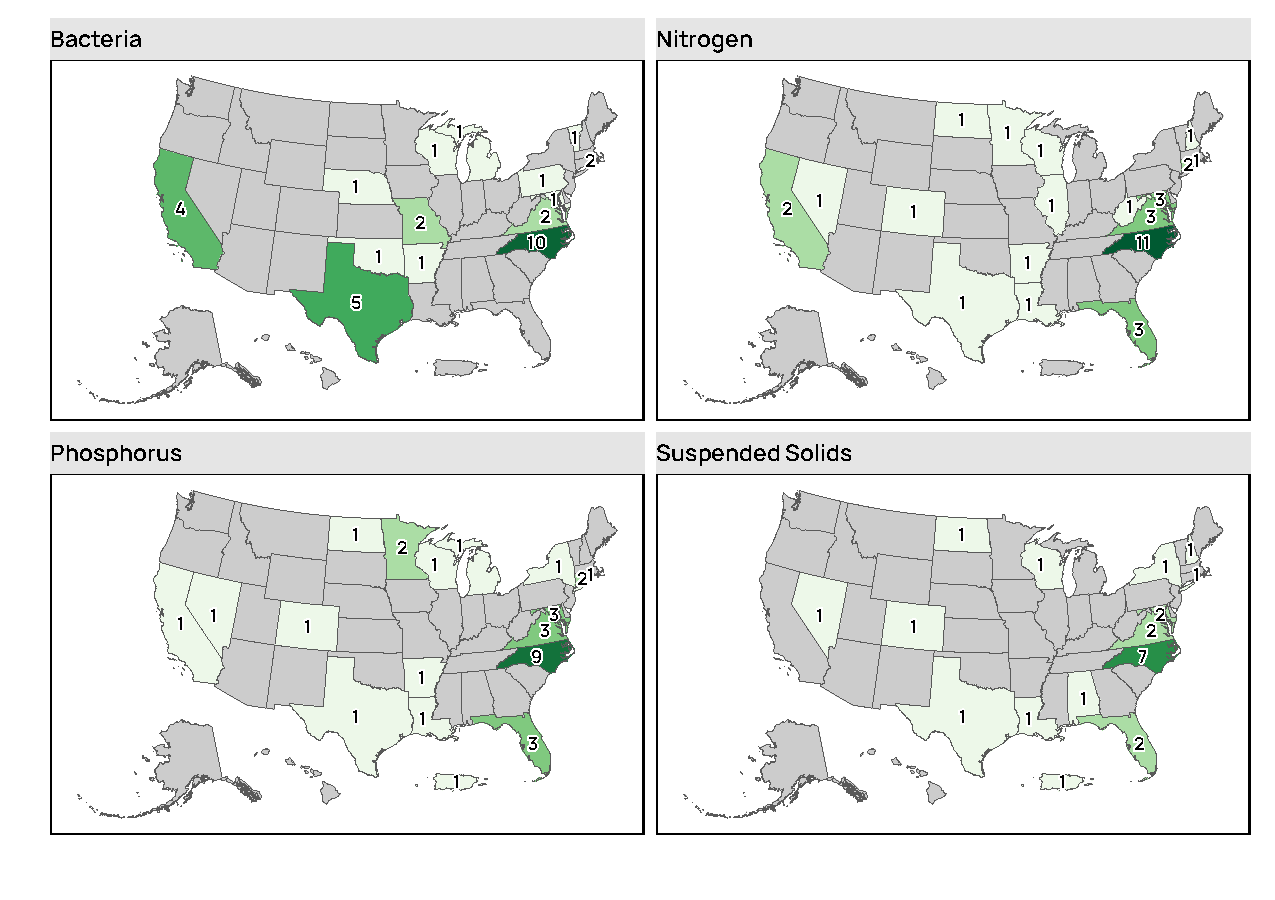
\includegraphics[width=1\linewidth,]{../figures/study_map} \caption{Distribution of studies identified in the systematic review by state and parameter.}\label{fig:studymap}
\end{figure}

\begin{figure}[p]
\includegraphics[width=1\linewidth,]{../figures/overall_effect} \caption{Estimated effect sizes and intervals from the intercept only multilevel random effects model. Individual points represent studies, with size scaled by sampling variance. The point estimate with uncertaintity bars indicate the estimated overall effect, 95\% confidence intervals, and 95\% prediction intervals. Here, \textit{k} indicates the number of overall effects with the number of unique studies in parenthesis.}\label{fig:overalleffect}
\end{figure}

\begin{figure}[p]
\includegraphics[width=1\linewidth,]{../figures/bac_predicted} \caption{Predicted marignal effect of influent FIB and aridity index (conditioned on BMP subcategory). Solid lines are the predicted mean effect, dashed lines are the 95\% confidence intervals, and the dotted lines are the 95\% prediction intervals. Individual dots represent each effect size identified in the literature with the size scaled by sampling variance.}\label{fig:fibeffect}
\end{figure}

\begin{figure}[p]
\includegraphics[width=1\linewidth,]{../figures/phos_predicted} \caption{Predicted marignal effect of influent pollutant concentration on TP (Panel A) and PO\textsubscript{4} (Panel B) reductions. Solid lines are the predicted mean effect, dashed lines are the 95\% confidence intervals, and the dotted lines are the 95\% prediction intervals. Individual dots represent each effect size identified in the literature with the size scaled by sampling variance.}\label{fig:phoseffect}
\end{figure}



\end{document}
